\documentclass{article}
\usepackage{graphicx} % Required for inserting images

\usepackage[french]{babel}
\usepackage[T1]{fontenc}
\usepackage{lmodern}
\usepackage{hyperref}
\usepackage{wrapfig}

\title{Rapport de projet : Chat201 – édition thread \& réseau}
\author{Daniel DEFOING (\texttt{ddef0003}) \and 
        Belinda ÖZNUR (\texttt{bozn0003}) \and
        Haluk YILMAZ (\texttt{hyil0003})}
\date{\today}

\begin{document}
\pagenumbering{gobble}

\maketitle
\tableofcontents
\newpage

\pagenumbering{arabic}
\section{Introduction}
Ce rapport décrit globalement la conception du second projet dans le cadre du cours de Systèmes d'Exploitation
(INFO-F201). Il présente les choix de conception qui ont guidé notre développement, et les difficultés qui ont pu survenir durant celui-ci. Pour voir de façon précise les changements ayant eu lieu tout au long du projet et la contribution de chacun, veuillez consulter \hyperref[https://github.com/Daniel-Dfg/OS_Projet_2]{le repository GitHub de notre projet}.

\section{Choix du langage :pourquoi C++ plutôt que C ?}

\subsection*{Des outils qui facilitent le développement en général}
Une raison fondamentale qui a guidé cette décision est que C++ possède des fonctionnalités absentes en C tels que les références, les chaînes de caractères (ou \textit{strings}, qu'on a souvent subsitués aux \texttt{char*[]}) ou encore les classes. 

On peut aussi parler des conteneurs STL comme \texttt{std::vector} ou \texttt{std::queue}, très utilisés dans cette implémentation du projet.

Or, dans le cadre du projet présenté ici, ces éléments apportent une pluvalue non négligeable en permettant de structurer un code de façon plus fine qu'en C ou de simplifier grandement certaines opérations. L'exemple le plus trivial qu'on peut donner de ceci est le passage de paramètres par référence plutôt que par pointeur dans certaines fonctions, qui permet une gestion plus sûre de la mémoire.

\subsection*{Des librairies qui fournissent des abstractions utiles pour ce projet}
On va illustrer ce point en parlant des \textit{threads}. En langage C, on utilisera \texttt{thread.h} pour les gérer, alors qu'en C++ on a par exemple accès à la librarie \texttt{std::thread}, qui permet d'abstraire certaines opérations de la librarie en C (par exemple, accéder au thread courant avec \texttt{std::this\_thread}).

Utiliser C++ permet donc l'usage de certaines libraries standard absentes en C qui permettent d'abstraire des opérations de libraries \textit{correspondantes} en C.

\subsection*{Pas de perte notable à ne pas utiliser le langage C}
C++ reste évidemment compatible avec C : il n'existe pas d'opération en C infaisable exactement de la même façon en C++.
De plus, les deux langages étant connus pour leur rapidité d'exécution, la performance du C++ n'est pas dégradée de façon significative par rapport au C dans le cadre de ce projet.

L'utiliser permet donc de tirer parti ses abstractions discutées plus haut (voir 2 sections précédentes) tout en gardant une très bonne efficacité.


Tout ceci montre que les avantages majeurs ont été trouvés à utiliser C++ plutôt que C, alors qu’aucun avantage n’a été identifié en faveur de l’utilisation de C par rapport à C++. Ce choix du langage s’est donc naturellement imposé comme le plus adapté.

\section{Visualisation de l'architecture du programme}
Cette section discute des choix de conception du programme final, des considérations qui permettront au lecteur de mieux comprendre la nature de ces choix et des problèmes rencontrés qui en ont suivi.

\subsection{Le serveur en tant que \textit{point relais} des clients}
La structure d'un programme client-serveur tel que celui présenté ici peut être visualisée très simplement sous la forme d'un Graphe Étoile \cite{Graphe Étoile}, avec le serveur au centre et les clients aux extrémités de chaque branche. 
\begin{figure}[ht]
    \centering
    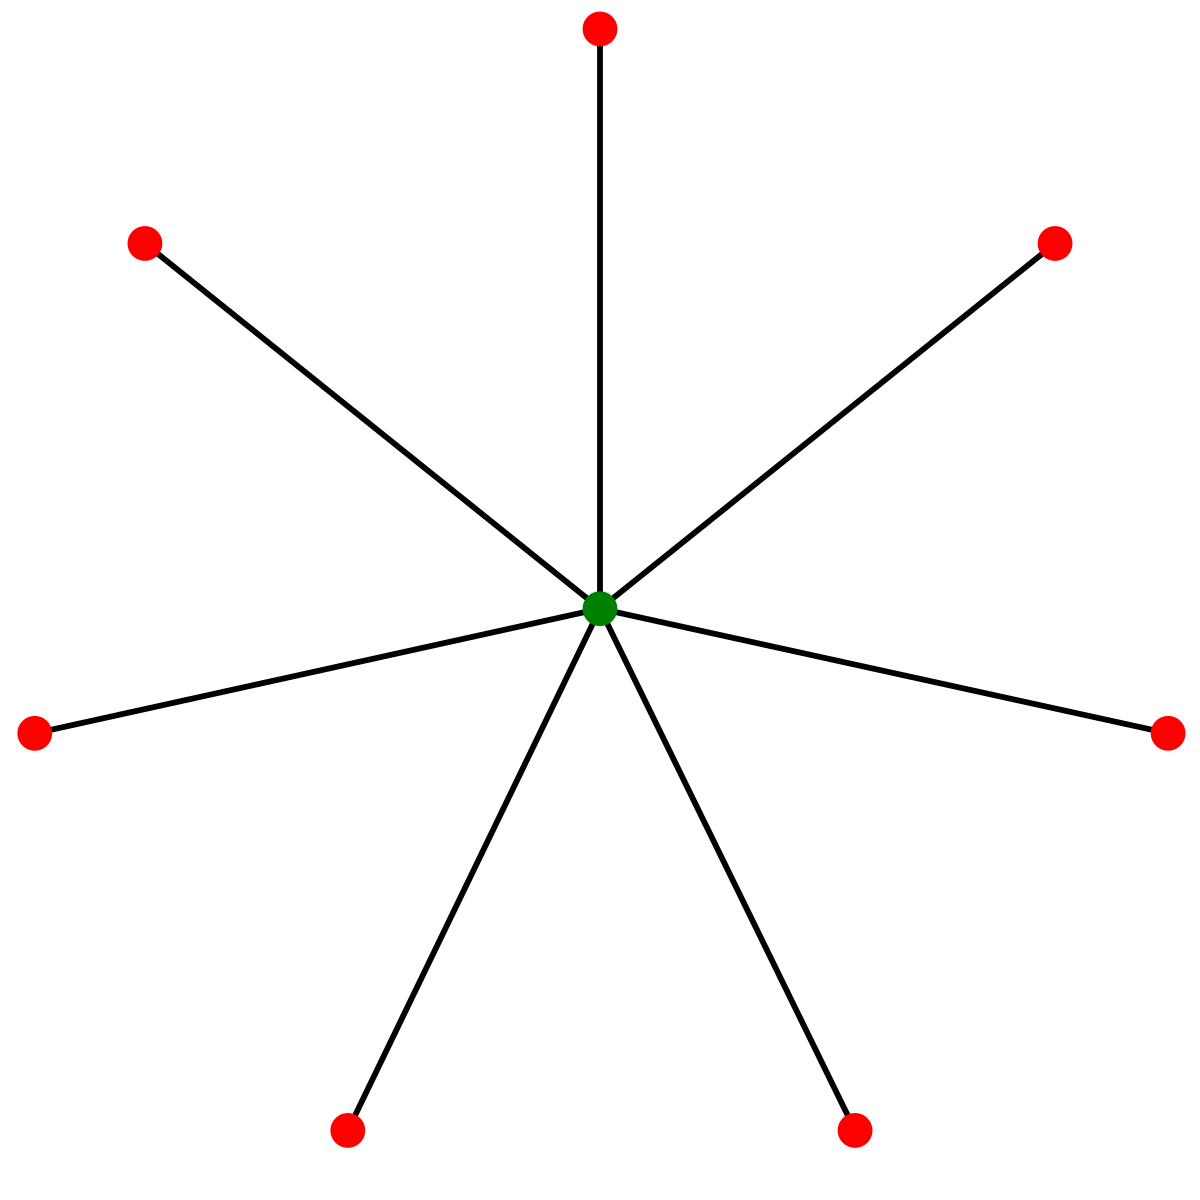
\includegraphics[width=0.25\linewidth]{etoile.png}
    \caption{\textit{Graphe Étoile typique.}}
\end{figure}

Cette représentation montre bien qu'un seul serveur se charge de \textit{relayer} les informations à passer d'un client à un autre ou d'un client vers lui-même (confirmation de (dé)connexion notamment). 

TODO : discuter du TCP/IP brièvement

Dans la suite, nous discuterons en profondeur de la façon dont les nœuds de ce graphe communiquent.

\subsection{Choix d'implémentation communs aux clients et au serveur}

\subsubsection{De la méthode d'envoi des messages}
Il a été décidé d'abstraire l'échange d'informations entre les clients et le serveur principalement par une classe \texttt{Message}. Un point très important qui découle de ce choix d'implémentation est qu'on a utilisé des \texttt{std::string} pour garantir une gestion dynamique de la mémoire et simplifier les opérations de manipulation des chaînes de caractère.

\subsection{Conception des clients}

\subsubsection{Deux FIFOs à vider en permanence}
Tout client possède deux \texttt{std::queue} qu'il observe en permanence: une pour les messages qu'ils envoie, et une pour celle qu'ils reçoit. 

Utilser des \texttt{std::queue} n'ayant pas de taille limitée ainsi est une partie de la solution aux problèmes de synchronisation qui peuvent être rencontrés dans le cadre de ce projet. 

En effet, si un client reçoit plusieurs messages en même temps, les messages peuvent être \textit{push} à l'arrière de la FIFO servant et traités séquentiellement par le client qui la videra progressivement.


 Mais n'y a-t-il pas un risque que, si on envoie plusieurs messages simultanément à un même client, les deux messages risquent de corrompre la FIFO de réception du client (qui est un objet critique) en voulant s'insérer dedans en même temps ?


En principe, oui, c'est un problème qui peut survenir si on ne prend pas de précaution contre lui. C'est pour cela qu'on a fait usage de mutex pour protéger la FIFO côté client (pour éviter que sa FIFO de réception reçoive plusieurs messages simultanément).


\subsubsection{Deux threads, deux FIFOs par client}
Ce point fait écho à la discussion de la section précédente sur l'usage de FIFOs côté client. 

Il faut préciser que le processus côté client se divise en deux \textit{threads}: un dédié à la réception des messages (qui doit donc vider et afficher le contenu de la FIFO de messages entrants) et un autre dédié à l'envoi de messages (qui doit donc en quelque sorte remplir la FIFO des messages à envoyer, puis la vider progressivement). 

Cette division du processus client en deux threads est due à des contraintes évidentes de performance et autorise le client à envoyer et recevoir des messages simultanément (gestion asynchrone des communications).

\subsubsection{Gestion de la (dé)connexion au serveur}
Tout client doit suivre le protocole TCP (réf. nécessaire) pour initialiser sa connexion et doit s'identifier auprès du serveur.
(incomplet)


 Gestion de la déconnexion (quel thread tue l'autre, comment on se déconnecte) TODO :
1. Signal de terminaison envoyé aux deux threads
2. Attente de la fin des opérations en cours
3. Libération des ressources
4. Fermeture propre de la connexion

\subsection{Conception du serveur}

\subsubsection{De l'utilisation de \texttt{poll}}
\texttt{poll} est l'outil qui a été choisi côté serveur pour gérer les connexions et envoi de messages par les clients. Il fonctionne ainsi : 
\begin{enumerate}
    \item Initialiser un \texttt{std::vector} de \texttt{pollfd} (autrement dit, un vecteur de descripteurs de fichier pour pouvoir établir les communications). 
    \item Chaque client qui se connecte au serveur lui fait ajouter une nouvelle entrée au \texttt{std::vector}. Symétriquement, lors d'une déconnexion, il faut le parcourir pour supprimer l'entrée dans le vecteur du client qui s'est déconnecté.
    \item Le serveur se charge de "surveiller" le vecteur de \texttt{pollfd} en permanence, en regardant pour chacun s'il y a un message à transmettre : en pratique, il \textit{boucle} sur le vecteur pendant toute sa durée de vie. 
    \item S'il observe que, dans un \texttt{pollfd}, il y a un message à transmettre, alors il recherche à qui le client envoyeur a voulu transmettre son message \footnote{En pratique, on recherche le nom du client récepteur dans un \texttt{std::unordered\_map} avec le nom du client comme clé et son \texttt{pollfd} comme valeur.} et, s'il existe, écrit dans le \texttt{pollfd} du client récepteur.

    Si le message à envoyer ne contient pas de nom de destinataire ou que le nom de destinataire spécifié ne fait référence à aucun client connecté, un message d'erreur est renvoyé. 
\end{enumerate}


\section{Améliorations non réalisées de l'implémentation actuelle}
\subsection{\texttt{epoll} comme alternative à \texttt{poll}}
\texttt{epoll} fonctionne de façon assez similaire à \texttt{poll}, mais a deux différences majeures:
\begin{enumerate}
    \item Il ne fonctionne que sur les systèmes d'exploitation Linux (ou basés sur Linux)
    \item Spécifier qu'il peut être edge-triggered ou level-triggered (et préciser le sens de tout ceci)
\end{enumerate}

En clair, \texttt{epoll} est cité comme une alternative plus rapide que \texttt{poll}, mais n'a pas été implémenté dans le cadre de ce projet car l'API est plus complexe à utiliser que celle de \texttt{poll}. Cela aurait tout à fait pu être fait en quelques jours supplémentaires cependant.

\subsection{Attente active pour les FIFOs côté client}
On l'a vu en section 3.3 (\ref{Conception des Clients}), tout client est séparé en deux threads dont l'un gère une FIFO pour les messages entrants et l'autre les messages sortants. Cependant, l'implémentation actuelle de ce projet fait que le contenu des FIFOs est vérifié en permanence tant que le client est connecté \footnote{On pourrait en quelque sorte parler d'\textit{attente active} de la part du client. }

Par manque de temps, un système plus propre n'a pas pu être mis en place, mais on peut en esquisser le fonctionnement théorique (qui aurait certainement pu, comme pour \texttt{epoll}, être implémenté en quelques jours) :
\begin{enumerate}
    \item Initialement, la FIFO des messages entrants est vide. Dès qu'un message est envoyé au client, celui-ci commence à vider la FIFO. 
    \item Chaque nouveau message entrant correspond à une nouvelle "notification" pour le client, à une nouvelle tâche à faire : on peut donc facilement avoir un "compteur de tâches à faire" qui indique combien de fois le client doit extraire un message de la FIFO. Par exemple, si un client reçoit 3 messages en même temps, il est censé être notifié 3 fois et donc extraire le premier élément de la FIFO 3 fois (ce qui vide exactement la FIFO, en principe). 
    \item Lorsque la FIFO est vide, le client n'a pas besoin de vérifier son contenu en permanence.
\end{enumerate}

\section{Difficultés rencontrées et solutions trouvées}
\subsection{Problèmes de synchronisation}
\begin{itemize}
    \item côté serveur, accès concurrents (problème producteur-consommateur)
    \item Signaux asynchrones (mentionner la conception du SignalManager dans l'explication de la solution)
    \item ...
\end{itemize}

\subsection{Garantie de l'intégrité du contenu partagé par les clients}
\begin{itemize}
    \item Gestion des tailles limites (longueur de pseudos et de messages)
    \item Comment s'est-on assurés que le messages étaient bien transmis sans perte ?
\end{itemize}


\begin{thebibliography}{999}
	\bibitem{Graphe Étoile}
		Wikipedia. (dernière modification : 2019, 21 janvier). \textit{Graphe étoile.} URL: \url{https://fr.wikipedia.org/wiki/Graphe_%C3%A9toile}, consulté le 12/12/2024.
\end{thebibliography}
\end{document}

